\section{Evaluation}
\label{sec:eval}
% Written in one pass from the eval-freeze-rc13 archive (repro/results, 9 Nov 2026). Every number is the median of
% three runs on the frozen build cf4d88ce; the tables and figures are generated by scripts/plot_sweep_results.py.

We ask four questions. How does the operator compare with Kuzu, Neo4j, Memgraph and FalkorDB, and with the two
other ways of answering the same question inside \duckdb, from one path to tens of thousands and on graphs of
different structure? What does the index add over building the CSR inside the query, and what does it cost to
create? How do the two routes behave when the graph changes under concurrent readers? And what does each mechanism
of Section~\ref{sec:operator} contribute?

\paragraph{Setup} All experiments run on one AWS m7a.8xlarge (32 AMD EPYC 9R14 cores, one thread per core, 128\,GiB
of memory, Amazon Linux 2023). \duckpgq runs on \duckdb v2.0.0-dev (commit 45f4fdf3), compiled with \duckdb's default
flags for x86-64-v3, so with AVX2, with every setting at its default and 32 threads. All measurements use this build; the
reproduction package names its commit. \rev{We compare with} Kuzu 0.11.3 (embedded, 32 threads)\footnote{Kuzu's repository was archived in 2025. Its maintained fork, LadybugDB 0.15.3,
was not faster than Kuzu 0.11.3 in our tests at SF10, between 1.1 and 2.9 times slower on the random-pair,
sources $\times$ all and LDBC points, so we report Kuzu.}, Neo4j 5.26.32 Enterprise (16\,GB heap, 16\,GB page cache, parallel runtime; the
GDS library 2.13.14 with its unlicensed limit of four threads where marked; Neo4j's store is 2.3\,GB at SF300, Table~\ref{tab:fixed-costs}, so the page cache holds it at every scale, and a check with a 31\,GB heap and a 64\,GB page cache changed Neo4j's SF300 times by less than two percent), and Memgraph 3.14.0 and FalkorDB 4.2.2
in Docker with their default configuration, both of which run a query on one thread. Two other ways of answering the same question inside \duckdb are included, the recursive CTE of plain SQL and the
2023 \duckpgq design, whose UDFs build the CSR and run \msbfs on one core per morsel of
input~\cite{tenwolde2023duckpgq}. ``\duckpgq build''
builds the partitioned CSR inside the query; ``\duckpgq index'' reads a CSR index created once before the first
query. The index of the sweep has no reverse partitions; Table~\ref{tab:ablation} measures what they add.

The graphs are the \texttt{Person\_knows\_Person} relation of LDBC SNB at scale factors 10, 100 and 300, with 1.84M,
18.7M and 55.7M edges stored once in the direction the generator produces them, and three Graphalytics
graphs~\cite{iosup2016graphalytics} of other structure, cit-Patents (3.8M vertices, 16.5M edges, a citation DAG in
which a source reaches about 2000 vertices), datagen-8\_4-fb (3.8M vertices, 269M undirected edges stored in both
directions, so dense that a source reaches the whole graph) and graph500-24 (8.9M vertices, 260M undirected edges,
with hubs). Every system loads the same snapshot, exported from the \duckdb tables as CSV, and as Parquet for Kuzu.
Random pairs, sources $\times$ all and the update workload traverse the stored direction; the LDBC queries use the
undirected closure of \texttt{knows}.

\emph{Random pairs} returns the hop-count shortest-path length of each of $n$ pairs taken from a fixed pseudo-random
sequence, so that the pairs for a smaller $n$ are a prefix of those for a larger one; on the directed \texttt{knows}
graph about half of them are reachable, on datagen and graph500-24 all of them, and on the citation DAG none, which is why cit-Patents runs only the second shape. The single pair sampled at SF100 is unreachable, so that point measures a full search of the source's component in every system. \emph{Sources $\times$ all} returns the distance from each of $k$
sampled sources to every reachable vertex, the shape of a reach query. Three LDBC queries have a shortest path at
their core, IC13 (one pair), BI19 (every pair between the persons of two cities) and BI20 (one target, every person
of one company); we run their hop-count variants with five parameter sets each. Each system runs each query in its own language in the formulation that was fastest for it, listed in the reproduction package, including the split of the pairs over 32 client connections where that was faster. The Cypher patterns
carry a hop bound of 30, Kuzu's default maximum, and \duckpgq's carry none; the counts agree on every point a bounded
system finishes, so the bound cut no path. A query over 600\,s is reported as timed out, and the larger points of the
same shape are then recorded as timed out without running them. Every point is the median of three runs; the LDBC
table reports the median of the three runs per parameter set, averaged over the five sets. A \duckpgq run is a fresh
process that executes the query once untimed, which also loads the index, before the timed runs; the native systems
run three timed repetitions back to back, and a cold first run does not move the median. Wherever two systems complete the same point, the harness finds the same number of reached pairs and the same sum
of path lengths.

\begin{figure}[t]
  \centering
  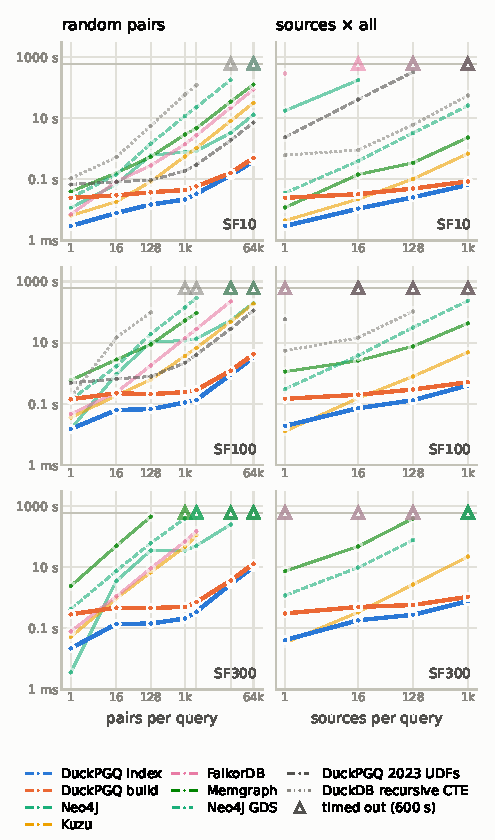
\includegraphics[width=\linewidth]{figures/scaling_column.pdf}
  \caption{Left: hop-count shortest-path length for $n$ random pairs in one query. Right: distance from each of $k$
  sources to every reachable person. LDBC SNB SF10, SF100 and SF300 from top to bottom; y: seconds per query, log
  scale, median of three runs, 32 threads. One line per system in its fastest formulation, the two \duckdb-native ways
  dashed in grey; a triangle marks a run over the 600\,s limit, after which the larger points were not run.}
  \label{fig:scaling}
\end{figure}

\subsection{One path or thousands}
\label{sec:eval-pairs}

For one pair the operator runs a single-source traversal (Section~\ref{sec:traversals}), and on a large graph
that is slower than a bidirectional search. At SF300 the index route takes 22\,ms for one pair and Neo4j 4\,ms (Figure~\ref{fig:scaling}). The sampled pair is five hops apart; the operator's five levels touch most of the graph
and take 18 to 20 of the 22\,ms, where Neo4j's bidirectional search meets in the middle after two or three levels
from each side. From one source to every person the operator is within 8\,ms of Kuzu, whose recursive join from a
literal source is a single-source search as well.

With more pairs the operator's time grows slowly, because it runs one search per distinct source and shares each
traversal among up to 256 of them. From one pair to 65\,536 at SF10 its time grows by a factor of 130. Kuzu, Neo4j,
FalkorDB and Memgraph answer a list of pairs one search at a time, and their time grows linearly with the pairs;
Neo4j, whose parallel runtime runs the searches side by side, is the fastest of the four. The operator is ahead of all
four from sixteen pairs on. At 65\,536 pairs on SF10 it is 33 times faster than Neo4j and 320 times faster than
Memgraph. At SF300 it answers 65\,536 pairs in 10.0\,s over the index, and none of the four finishes within the
limit; Neo4j is the last to exceed it, after 248\,s for 16\,384 pairs.

In reach mode, the distance from each source to every reachable person, the operator shares its traversals in the
same way. At 1024 sources on SF300 it produces 530\,M distances in 773\,ms over the index, 28 times faster than Kuzu,
which runs one search per source, as Neo4j GDS does. Neo4j's Cypher and FalkorDB have no single-source form; they run
one \texttt{shortestPath} per destination and exceed the limit already at one source from SF100 on.

Inside \duckdb the operator replaces the 2023 UDFs and the recursive CTE. The UDFs receive their work per tuple and run one query on one core. They stay an order of magnitude
behind the operator on random pairs, and on sources $\times$ all, where they must enumerate every destination as a
pair, they need 2.4\,s for one source at SF10 where reach mode needs 3\,ms. The recursive CTE evaluates a join per
step and exceeds the limit from 16\,384 pairs at SF10.

\begin{table}[t]\centering\scriptsize\setlength{\tabcolsep}{3pt}
\caption{Three Graphalytics graphs: seconds per query for $k$ sources to every reachable vertex and for 65\,536 random pairs (none on the citation DAG is reachable); median of three runs, 32 threads, fastest formulation.}\label{tab:graphalytics}
\begin{tabular}{lrrrrr}\toprule
system & 1 source & 16 & 128 & 1024 & 65\,536 pairs \\ \midrule
\multicolumn{6}{l}{\textit{cit-Patents: 3.8M V, 16.5M E, directed, deep levels}} \\
\quad DuckPGQ index & 32\,ms & 104\,ms & 172\,ms & \textbf{437\,ms} & -- \\
\quad DuckPGQ build & 141\,ms & 231\,ms & 270\,ms & 502\,ms & -- \\
\quad Neo4j & 27.2\,s & 309\,s & timeout & timeout & -- \\
\quad Kuzu & 7\,ms & 71\,ms & 299\,ms & 1.5\,s & -- \\
\quad FalkorDB & timeout & timeout & timeout & timeout & -- \\
\quad Memgraph & \textbf{4\,ms} & \textbf{48\,ms} & \textbf{127\,ms} & 498\,ms & -- \\
\quad Neo4j GDS (4 thr.) & 68\,ms & 1.0\,s & 8.3\,s & 66.7\,s & -- \\
\addlinespace
\multicolumn{6}{l}{\textit{graph500-24: 8.9M V, 521M E, hubs}} \\
\quad DuckPGQ index & 351\,ms & \textbf{4.5\,s} & \textbf{2.7\,s} & \textbf{8.8\,s} & \textbf{144\,s} \\
\quad DuckPGQ build & 2.8\,s & 7.0\,s & 5.6\,s & 10.8\,s & 148\,s \\
\quad Kuzu & \textbf{336\,ms} & 8.1\,s & 61.6\,s & 495\,s & timeout \\
\addlinespace
\multicolumn{6}{l}{\textit{datagen-8\_4-fb: 3.8M V, 539M E, dense}} \\
\quad DuckPGQ index & \textbf{175\,ms} & \textbf{1.9\,s} & \textbf{1.1\,s} & \textbf{4.1\,s} & \textbf{51.0\,s} \\
\quad DuckPGQ build & 2.7\,s & 4.5\,s & 3.9\,s & 6.8\,s & 53.3\,s \\
\quad Kuzu & 189\,ms & 3.0\,s & 24.0\,s & 191\,s & timeout \\
\bottomrule\end{tabular}\end{table}


\paragraph{Graph structure} Table~\ref{tab:graphalytics} repeats sources $\times$ all on three Graphalytics graphs, with Kuzu on all
three and every system on cit-Patents. How much the operator gains from sharing depends on the part of the graph a
search covers. On cit-Patents a source reaches about 2000 of 3.8M vertices, and a search per source is cheap. The
operator loses the one-source point to Memgraph and Kuzu, 32\,ms against 4 and 7\,ms, and at 1024 sources it leads
Memgraph by 14\,\% and Kuzu by 3 times. On datagen and graph500-24 a source reaches the whole graph. The operator ties
with Kuzu at one source and is 47 and 56 times faster at 1024, and on random pairs Kuzu exceeds the limit from 16\,384
and from 2048 pairs. On both graphs the operator is slower for 16 sources than for 128 (4.5 against 2.7\,s on
graph500-24), because its few-sources rule sends 16 sources to the single-source traversal, each search sweeping 4 to
9\,M vertices, while 128 run as lanes. The default of 16 fits \texttt{knows}, and Section~\ref{sec:choice} shows that
the crossover is a property of the graph. None of the six graphs has a high diameter, such as a road network.

\subsection{LDBC queries}
\label{sec:eval-ldbc}

\begin{table*}[t]\centering\scriptsize\setlength{\tabcolsep}{4pt}
\caption{LDBC IC13 (one pair), BI19 (city $\times$ city) and BI20 (company $\to$ one person) as hop-count shortest paths on the undirected knows graph: seconds per query, the median of three runs per parameter set averaged over five sets, 32 threads, each system in its fastest formulation.}\label{tab:ldbc}
\begin{tabular}{lrrrrrrrrr}\toprule
 & \multicolumn{3}{c}{LDBC SF10} & \multicolumn{3}{c}{LDBC SF100} & \multicolumn{3}{c}{LDBC SF300} \\
system & IC13 & BI19 & BI20 & IC13 & BI19 & BI20 & IC13 & BI19 & BI20 \\ \midrule
DuckPGQ index & 4\,ms & \textbf{12\,ms} & \textbf{5\,ms} & 14\,ms & \textbf{137\,ms} & \textbf{26\,ms} & 28\,ms & \textbf{765\,ms} & \textbf{61\,ms} \\
DuckPGQ build & 33\,ms & 44\,ms & 37\,ms & 267\,ms & 423\,ms & 288\,ms & 626\,ms & 1.6\,s & 692\,ms \\
Neo4j & \textbf{3\,ms} & 40\,ms & 22\,ms & \textbf{7\,ms} & 3.9\,s & 126\,ms & \textbf{6\,ms} & 47.0\,s & 1.2\,s \\
Kuzu & 7\,ms & 524\,ms & 1.4\,s & 24\,ms & 22.3\,s & 29.4\,s & 50\,ms & 332\,s & timeout \\
FalkorDB & 12\,ms & 18.4\,s & 2.9\,s & 52\,ms & timeout & 212\,s & 116\,ms & timeout & timeout \\
Memgraph & 375\,ms & 140\,ms & 97\,ms & 8.6\,s & 17.0\,s & 646\,ms & 31.8\,s & timeout & 47.8\,s \\
Neo4j GDS (4 thr.) & 69\,ms & 11.0\,s & 66.9\,s & 530\,ms & timeout & timeout & 1.5\,s & timeout & timeout \\
\bottomrule\end{tabular}\end{table*}


Table~\ref{tab:ldbc} repeats the comparison on three queries of the LDBC Social Network
Benchmark~\cite{erling2015ldbc,puroja2023ldbcv2,szarnyas2022ldbcbi} that have a shortest path at their core. The result of each follows from the shape of its pairs. IC13 asks for one pair, and Neo4j is the fastest system at every scale. Its
bidirectional search explores a small neighbourhood of both endpoints, and takes 3 to 7\,ms at every scale. The operator's single-source traversal expands whole levels from one side, and its time grows with the graph, from 4\,ms at SF10 to 28\,ms at SF300. BI19 (Figure~\ref{fig:teaser}) asks for the distance between every person of one city and every
person of another. Its pairs grow with the product of the two cities, to 2.4\,M per query at SF300, but its distinct
sources grow only with one city, to about 1400, which the operator runs as six batches. A system that searches once per pair does work in proportion to the pairs. Neo4j therefore takes 3 times as long as the index route at SF10, 28 times at SF100 and 61 times at SF300; at SF300 Kuzu needs 332\,s, and Memgraph, FalkorDB and Neo4j GDS exceed the limit.
BI20 is the opposite shape, the distance from every person of one company to one target, and its pairs share a destination where BI19's share sources. The index of the sweep has no reverse partitions and runs one search per source, and is still 4 to 20 times faster than Neo4j; with reverse partitions the operator runs a single search from the target
(Section~\ref{sec:choice}), 6 against 116\,ms for 1024 sources at SF100 (Table~\ref{tab:ablation}).

\subsection{Index or build}
\label{sec:eval-index}

\begin{table}[t]\centering\scriptsize\setlength{\tabcolsep}{2.5pt}
\caption{Fixed costs per graph, 32 threads: creating the CSR index over the loaded edge table and its size per edge, against the native systems' import from the same CSV files (Kuzu from Parquet) and Kuzu's store size per edge. Memgraph, FalkorDB and Neo4j were not loaded with the two large Graphalytics graphs.}\label{tab:fixed-costs}
\begin{tabular}{lrrrrrrrr}\toprule
graph & edges & \multicolumn{2}{c}{CSR index} & \multicolumn{2}{c}{Kuzu} & Neo4j & Memgraph & FalkorDB \\
 & & create & B/edge & import & B/edge & import & import & import \\ \midrule
SNB SF10 & 1.8\,M & 0.13\,s & 11.4 & 1.2\,s & 31 & 24\,s & 6.8\,s & 85\,s \\
SNB SF100 & 18.7\,M & 1.3\,s & 10.9 & 3.6\,s & 24 & 4\,min & 89\,s & 15\,min \\
SNB SF300 & 55.7\,M & 4.5\,s & 11.1 & 8.8\,s & 24 & 14\,min & 4\,min & 43\,min \\
cit-Patents & 16.5\,M & 0.98\,s & 17.1 & 2.8\,s & 24 & 4\,min & 88\,s & 13\,min \\
datagen-8\_4-fb & 539.0\,M & 60\,s & 11.6 & 69\,s & 16 & -- & -- & -- \\
graph500-24 & 520.8\,M & 50\,s & 12.9 & 68\,s & 18 & -- & -- & -- \\
\bottomrule\end{tabular}\end{table}

\begin{table}[t]\centering\scriptsize\setlength{\tabcolsep}{3pt}
\caption{Random pairs over three CSRs of the same layout that differ in whether they are built inside the query and in how they number vertices; seconds per query, median of three runs, 32 threads. The two indexes were measured on copies of the sweep's databases.}\label{tab:numbering}
\begin{tabular}{llrrrr}\toprule
 & & \multicolumn{4}{c}{seconds per query} \\
 & & \multicolumn{2}{c}{SF100} & \multicolumn{2}{c}{SF300} \\
CSR & vertex ids & 2048 & 65\,536 & 2048 & 65\,536 \\ \midrule
built per query (build route) & row order & 0.283 & 4.1 & 0.714 & 12.8 \\
index keyed by row ids & row order & 0.147 & 4.0 & 0.407 & 12.1 \\
index keyed by person ids & sorted keys & 0.129 & 3.3 & 0.343 & 9.8 \\
\bottomrule\end{tabular}\end{table}


The index route is faster than the build route on every point of Figure~\ref{fig:scaling}, and on large queries
by more than the build it saves. For one pair the difference is the build of the CSR, which takes 22, 126 and
263\,ms at SF10, SF100 and SF300 and is nearly the whole query on the build route. Up to 2048 pairs the difference
stays close to that. At 65\,536 pairs it is 2.8\,s at SF300, ten times the build.

The cause is the numbering of the vertices. Both routes traverse a CSR of the same layout, built by the same code,
but the build route numbers the vertices by their row in the person table and the index by the sorted order of their
keys. To separate the numbering from the build we created a second index keyed by the persons' row ids, which has the
build route's numbering and no build (Table~\ref{tab:numbering}). For 65\,536 pairs at SF300 it takes 12.1\,s, which
is 0.7\,s less than the build route, about the build, and 2.3\,s more than the index on keys. The numbering therefore
accounts for most of the index's lead on large queries. We attribute it to locality: the traversal's per-vertex state
is read and written in id order, and ids that follow the keys keep those accesses closer together.

Table~\ref{tab:fixed-costs} gives what the index costs before the first query. Creating it is one partitioned
CSR build over the whole table plus the dictionary and a row id per edge, at 9 to 15 million edges per second: 4.5\,s
at SF300 and about a minute on the two Graphalytics graphs of 520 to 540\,M edges. The index takes 11 to 13 bytes per
edge, 8 of them the row id, and 17 on cit-Patents, whose 4.4 edges per vertex make the sparse rows a larger share;
Kuzu's store takes 16 to 31 bytes per edge. Importing the same data takes Kuzu 2 to 9 times as long as creating the index, and takes
Neo4j and FalkorDB 14 and 43 minutes at SF300. After a restart the index is loaded on the first query, in 117\,ms at
SF300 and under a second on the large graphs when the database file is in the page cache, and otherwise at the
volume's 270\,MB/s, 2.1\,s at SF300.

\subsection{Updates and concurrent readers}
\label{sec:eval-updates}

\begin{table}[t]\centering\scriptsize\setlength{\tabcolsep}{3pt}
\caption{The update stream at SF10, 190 commits of 2000 edge changes with one query after each, 32 threads: query latency for one source to 1024 destinations and for 1024 random pairs (median and p99 over the 190 queries) and the writer's median commit; the fastest cell per column in bold.}\label{tab:updates}
\begin{tabular}{lrrrrr}\toprule
 & \multicolumn{4}{c}{query latency (ms)} & commit (ms) \\
 & \multicolumn{2}{c}{1 source $\to$ 1024 dest.} & \multicolumn{2}{c}{1024 random pairs} & \\
system & median & p99 & median & p99 & median \\ \midrule
\multicolumn{6}{l}{\textit{DuckPGQ}} \\
\quad index, automatic folds & \textbf{15} & 31 & \textbf{44} & \textbf{56} & \textbf{19} \\
\quad index, no fold & 19 & 38 & 50 & 70 & \textbf{19} \\
\quad index, visibility per row & 35 & 65 & 65 & 93 & \textbf{19} \\
\quad build & 20 & 25 & 54 & 59 & \textbf{19} \\
\addlinespace
Kuzu & 17 & \textbf{24} & 6\,762 & 8\,056 & 335 \\
Memgraph & 43 & 48 & 47\,102 & 47\,822 & 27 \\
Neo4j & 1\,481 & 1\,631 & 743 & 819 & 66 \\
FalkorDB & 9\,423 & 9\,851 & 8\,683 & 8\,790 & 108 \\
\bottomrule\end{tabular}\end{table}


Table~\ref{tab:updates} compares the systems under the LDBC update stream for \texttt{knows} at SF10, applied
as 190 commits of 2000 edge changes with one query after each. A commit costs \duckdb 19\,ms with the index and
without it, because the index only appends the changed rows to its log; \rev{the other systems} need 27\,ms (Memgraph) to 335\,ms (Kuzu). The query over the index takes 15\,ms for one source to 1024 destinations, as fast as Kuzu and the
build route, and 44\,ms for 1024 random pairs, where \rev{the other systems} need 0.7 to 47\,s. Two rows of the table isolate the index's design; without folds the median rises from 15 to 19\,ms, the cost of a growing overlay, and with visibility
decided per log entry instead of per change group it rises to 35\,ms. The stream crosses the fold threshold, a tenth of
the epoch's edges by default (Section~\ref{sec:index-fold}), once, and the query that triggers the fold pays for it,
125\,ms where the others take 15\,ms.

\begin{figure}[t]
  \centering
  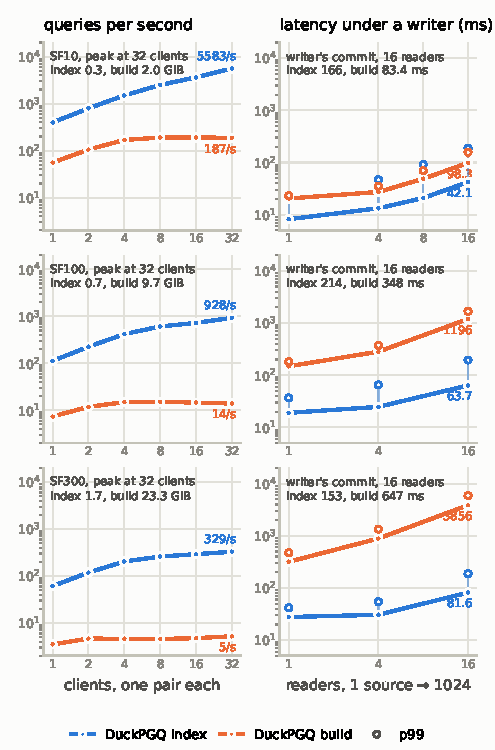
\includegraphics[width=\linewidth]{figures/concurrency_column.pdf}
  \caption{Left: queries per second for one random pair per query from 1 to 32 clients on one \duckdb instance with
  32 threads, over the index and building the CSR per query, with the process's peak memory at 32 clients. Right: latency of one source to 1024 destinations for 1, 4 and 16 readers while a writer commits 2000 edge
  changes every 200\,ms; the line is the median, the hollow marker the p99, the text the writer's median commit under each route's readers. SF10, SF100 and SF300 from top to bottom; log scales.}
  \label{fig:concurrency}
\end{figure}

Under concurrent readers the index's lead grows with the graph and with the readers
(Figure~\ref{fig:concurrency}). With one writer and 16 readers at SF300 a query takes 82\,ms over the index and
3.9\,s on the build route, 47 times as long, because every reader on the build route builds its own CSR of 55.7\,M
edges and sixteen builds compete for 32 cores; the build route's latency is about the build cost times the readers.
The same holds at SF100, 64\,ms against 1.2\,s, and with a smaller build at SF10, 42 against 98\,ms. The builds also
take memory, 17.8\,GiB against 6.0\,GiB at SF300, and time from the writer, whose commit takes 647\,ms under the build
route's readers and 153\,ms under the index's; at SF10 the order of the two commits is reversed, 166 against 83\,ms.
Throughput shows the same from the other side; from 1 to 32 clients the index route's single-pair throughput rises
from 61 to 329 queries per second at SF300, while the build route stays at 5, bound by its builds, and holds
23.3\,GiB against 1.7\,GiB, one CSR per client.

A fold is paid by one reader; at SF300 it takes 1.6 to 1.8\,s, a tenth of it the parallel scan of the table and
the rest the CSR build. In a run with the threshold lowered to 0.05\,\% of the edges, in which twenty commits caused
four folds, the four queries that triggered them took 1.7 to 1.8\,s, while the median of all sixteen readers stayed at
65\,ms and the p99 at 277\,ms. \rev{Under these loads every reader also answered its query a second time, over a CSR built from its own transaction's view of the table (Section~\ref{sec:index-correctness}). The two answers agreed in all 5376 queries, at the three scale factors and across folds.}

\subsection{What each mechanism contributes}
\label{sec:eval-ablation}

\begin{table}[t]\centering\scriptsize\setlength{\tabcolsep}{2.6pt}
\caption{One mechanism switched off or changed at a time, over the index at SF100, 32 threads unless stated: median seconds per query of three runs for one random pair, 2048 and 65\,536 random pairs, one source and 1024 sources to every reachable person, and 1024 sources to one destination. The index of the sweep has no reverse partitions; the row that adds them is the exception.}\label{tab:ablation}
\begin{tabular}{lrrrrrr}\toprule
 & \multicolumn{3}{c}{random pairs} & \multicolumn{2}{c}{sources $\times$ all} & $\to$ 1 \\
configuration & 1 & 2048 & 65\,536 & 1 & 1024 & 1024 \\ \midrule
default, 32 threads & 15\,ms & 135\,ms & 3.3\,s & 19\,ms & 421\,ms & 116\,ms \\
single-source traversal for every query & 15\,ms & -- & 39.1\,s & 19\,ms & 1.1\,s & 1.1\,s \\
multi-source traversal for every query & 15\,ms & -- & 3.3\,s & 19\,ms & 397\,ms & 118\,ms \\
pairs not grouped by source & 24\,ms & 520\,ms & 3.3\,s & 19\,ms & 410\,ms & 284\,ms \\
batches not grouped by the scheduler & 15\,ms & 258\,ms & 7.9\,s & 19\,ms & 377\,ms & 151\,ms \\
one batch at a time & -- & 814\,ms & 26.7\,s & -- & -- & -- \\
no summary bitmap & -- & 167\,ms & 4.2\,s & -- & -- & -- \\
destination ranges of 4096 & -- & 193\,ms & 6.0\,s & 18\,ms & 335\,ms & -- \\
with reverse partitions & 15\,ms & -- & 3.3\,s & 18\,ms & 419\,ms & 6\,ms \\
sources $\times$ all as a pair list & 15\,ms & -- & 3.3\,s & 83\,ms & 31.7\,s & 117\,ms \\
reach as one search per source & 15\,ms & -- & 3.3\,s & 19\,ms & 1.1\,s & 117\,ms \\
paths instead of lengths & 18\,ms & 1.6\,s & 45.9\,s & 19\,ms & 433\,ms & 1.3\,s \\
1 thread & 25\,ms & -- & 76.5\,s & 43\,ms & 4.6\,s & 1.3\,s \\
\bottomrule\end{tabular}\end{table}


Table~\ref{tab:ablation} changes one mechanism of the operator at a time, over the index at SF100. The largest effect is the choice of traversal; with the single-source traversal forced, 65\,536 pairs take twelve times as long
and 1024 sources 2.7 times, because every source then sweeps the graph on its own; with the multi-source traversal
forced nothing changes on these points, and Figure~\ref{fig:crossover} shows where it would. One lane per pair, as before the sources were deduplicated, takes 3.9 times as long for 2048 random pairs and 2.4 times for 1024 sources to one destination.
The scheduling of the batches comes second; without the grouping every batch is scheduled as an event of its own, 65\,536 pairs take 2.4 times as long, and on graph500-24 the working sets exceed the machine's memory, 98\,GiB against 32\,GiB. One batch at a time is eight times slower (nine times at SF10, 3.9 times at SF300), because threads idle whenever a level waits for its last task (Section~\ref{sec:phases}). The layout matters less; the summary bitmap saves 27\,\% at 65\,536 pairs, and destination ranges of 4096 instead of 65\,535 ids cost 1.8 times, because a sixteenth of the edges per partition means sixteen
times the partitions per level. The remaining rows are about what a query asks for. Sources $\times$ all as an
explicit pair list takes 75 times as long as reach mode for 1024 sources, and reverse partitions turn 1024 sources to
one destination into one search from the destination, 6\,ms against 116\,ms. Paths cost 14 times the lengths at 65\,536
pairs, because the operator runs paths as one search per source (Section~\ref{sec:traversals}); with paths it still
answers 65\,536 pairs in 45.9\,s, where Neo4j needs 199\,s for the lengths alone. On 32 threads the operator is 23
times faster than on one for 65\,536 pairs and 11 times for 1024 sources. One pair gains little from threads, because a
single-source traversal parallelizes only its dense levels.
